\documentclass{article}


% \usepackage{arxiv} # uncomment for preprint

\usepackage[utf8]{inputenc} % allow utf-8 input
\usepackage[T1]{fontenc}    % use 8-bit T1 fonts
% \usepackage{hyperref}       % hyperlinks
\usepackage{url}            % simple URL typesetting
\usepackage{booktabs}       % professional-quality tables
\usepackage{amsfonts}       % blackboard math symbols
\usepackage{nicefrac}       % compact symbols for 1/2, etc.
\usepackage{microtype}      % microtypography
\usepackage{lipsum}
\usepackage{graphicx}
\usepackage{subfigure}
\usepackage{amsmath}

\usepackage{placeins}
% \usepackage{algpseudocode}
\usepackage{algorithm}

% \algnewcommand\algorithmicforeach{\textbf{foreach}}
% \algdef{S}[FOR]{ForEach}[1]{\algorithmicforeach\ #1\ \algorithmicdo}


\usepackage{hyperref}

% Use the following line for the initial blind version submitted for review:
\usepackage{icml2021}

\begin{document}

\renewcommand{\thetable}{S\arabic{table}}

\renewcommand{\thefigure}{S\arabic{figure}}

\section{Datasets}
\label{supplement:sec:datasets}

Here we describe the datasets we use for benchmarks.
See Table~\ref{supplement:table:datasets} for a summary of this information.

The \textbf{annthyroid} dataset is derived from the ``Thyroid Disease'' dataset from the UCIMLR\@.
The original data has 7200 instances with 15 categorical attributes and 6 real-valued attributes.
The class labels are ``normal'', ``hypothyroid'', and ``subnormal''.
For anomaly detection, the ``hypothyroid'' and ``subnormal'' classes are combined into 534 outlier instances, and only the 6 real-valued attributes are used.

The \textbf{arrhythmia} dataset is derived from the ``Arrhythmia'' dataset from the UCIMLR\@.
The original dataset contains 452 instances with 279 attributes.
There are five categorical attributes which are discarded, leaving this as a 274-dimensional dataset.
The instances are divided into 16 classes.
The eight smallest classes collectively contain 66 instances and are combined into the outlier class.

The \textbf{breastw} dataset is also derived from the ``Breast Cancer Wisconsin (Original)`` dataset.
This is a 9-dimensional dataset containing 683 instances of which 239 represent malignant tumors and are treated as the outlier class.

The \textbf{cardio} dataset is derived from the ``Cardiotocography'' dataset.
The dataset is composed of measurements of fetal heart rate and uterine contraction features on cardiotocograms.
The are each labeled ``normal'', ``suspect'', and ``pathologic'' by expert obstetricians.
For anomaly detection, the ``normal'' class forms the inliers, the ``suspect'' class is discarded, and the ``pathologic'' class is downsampled to 176 instances forming the outliers.
This leaves us with 1831 instances with 21 attributes in the dataset.

The \textbf{cover} dataset is derived from the ``Covertype'' dataset.
The original dataset contains 581,012 instances with 54 attributes.
The dataset is used to predict the type of forest cover solely from cartographic variables.
The instances are labeled into seven different classes.
For outlier detection, we use only the 10 quantitative attributes as the features.
We treat class 2 (lodgepole pine) as the inliers, and class 4 (cottonwood/willow) as the outliers.
The remaining classes are discarded.
This leaves us with a 10-dimensional dataset with 286,048 instances of which 2,747 are outliers.

The \textbf{glass} dataset is derived from the ``Glass Identification'' dataset.
The study of classification of types of glass was motivated by criminological investigations where glass fragments left at crime scenes were used as evidence.
This dataset contains 214 instances with 9 attributes.
While there are several different types of glass in this dataset, class 6 is a clear minority with only 9 instances and, as such, points in class 6 are treated as the outliers while all other classes are treated as inliers.

The \textbf{http} dataset is derived from the original ``KDD Cup 1999'' dataset.
It contains 41 attributes (34 continuous and 7 categorical) which are reduced to 4 attributes (service, duration, src\_bytes, dst\_bytes).
Only the ``service'' attribute is categorical, dividing the data into \{http, smtp, ftp, ftp\_data, others\} subsets.
Here, only the ``http'' data is used.
The values of the continuous attributes are centered around 0, so they have been log-transformed far away from 0.
The original data contains 3,925,651 attacks in 4,898,431 records.
This smaller dataset is created with only 2,211 attacks in 567,479 records.

The \textbf{ionosphere} dataset is derived from the ``Ionosphere'' dataset.
It consists of 351 instances with 34 attributes.
One of the attributes is always 0 and, so, is discarded, leaving us with a 33-dimensional dataset.
The data come from radar measurements of the ionosphere from a system located in Goose Bay, Labrador.
The data are classified into ``good'' if the radar returns evidence of some type of structure in the ionosphere, and ``bad'' otherwise.
The ``good'' class serves as the inliers and the ``bad'' class serves as the outliers.

The \textbf{lympho} dataset is derived from the ``Lymphography'' dataset.
The data contain 148 instances with 18 attributes.
The instances are labeled ``normal find'', ``metastases'', ``malign lymph'', and ``fibrosis''.
The two minority classes only contain a total of six instances, and are combined to form the outliers.
The remaining 142 instances form the inliers.

The \textbf{mammography} dataset is derived from the original ``Mammography'' dataset provided by Aleksandar Lazarevic.
Its goal is to use x-ray images of human breasts to find calcified tissue as an early sign of breast cancer.
As such, the ``calcification'' class is considered as the outlier class while the ``non-calcification'' class is the inliers.
We have 11,183 instances with 6 attributes, of which 260 are ``calcifications.''

The \textbf{mnist} dataset is derived from the classic ``MNIST'' dataset of handwritten digits.
Digit-zero is considered the inlier class while 700 images of digit-six are the outliers.
Furthermore, 100 pixels are randomly selected as features from the original 784 pixels.

The \textbf{musk} dataset is derived from its namesake in the UCIMLR\@.
It is created from molecules that have been classified by experts as ``musk'' or ``non-musk''.
The data are downsampled to 3,062 instances with 166 attributes.
The ``musk'' class forms the outliers while the ``non-musk'' class forms the inliers.

The \textbf{optdigits} dataset is derived from the ``Optical Recognition of Handwritten Digits'' dataset.
Digits 1--9 form the inliers while 150 samples of digit-zero form the outliers.
This gives us a dataset of 5,216 instances with 64 attributes.

The \textbf{pendigits} dataset is derived from the ``Pen-Based Recognition of Handwritten Digits'' dataset from the UCI Machine Learning Repository.
The original collection of handwritten samples is reduced to 6,870 points, of which 156 are outliers.

The \textbf{pima} dataset is derived from the ``Pima Indians Diabetes'' dataset.
The original dataset presents a binary classification problem to detect diabetes.
This subset was restricted to female patients at least 21 years old of Pima Indian heritage.

The \textbf{satellite} dataset is derived from the ``Statlog (Landsat Satellite)'' dataset.
The smallest three classes (2, 4, and 5) are combined to form the outlier class while the other classes are combined to form the inlier class.
The train and test subsets are combined to produce a of 6,435 instances with 36 attributes.

The \textbf{satimage-2} dataset is also derived from the ``Satlog (Landsat Satellite)'' dataset.
Class 2 is downsampled to 71 instances that are treated as outliers, while all other classes are combined to form an inlier class.
This gives us 5,803 instances with 36 attributes.

The \textbf{shuttle} dataset is derived from the ``Statlog (Shuttle)'' dataset.
There are seven classes in the original dataset.
Here, class 4 is discarded, class 1 is treated as the inliers and the remaining classes, which are comparatively small, are combined into an outlier class.
This gives us 49,097 instances with 9 attributes, of which 3,511 are outliers.

The \textbf{smtp} is also derived from the ``KDD Cup 1999'' dataset.
It is pre-processed in the same way as the \textbf{http} dataset, except that the ``smtp'' service subset is used.
This version of the dataset only contains 95,156 instances with 3 attributes, of which 30 instances are outliers.

The \textbf{thyroid} dataset is also derived from the ``Thyroid Disease'' dataset.
The attribute selection is the same as for the \textbf{annthyroid} dataset but only the 3,772 training instances are used in this version.
The ``hyperfunction'' class, containing 93 instances, is treated as the outlier class, while the other two classes are combined to form an inlier class.

The \textbf{vertebral} dataset is derived from the ``Vertebral Column'' dataset.
6 attributes are derived to represent the shape and orientation of the pelvis and lumbar spine.
These attributes are: pelvic incidence, pelvic tilt, lumbar lordosis angle, sacral slope, pelvic radius and grade of spondylolisthesis.
Each instance comes from a different patient.
The ``Abnormal (AB)'' class of 210 instances are used as inliers while the ``Normal (NO)'' class is downsampled to 30 instances to be used as outliers.

The \textbf{vowels} dataset is derived from the ``Japanese Vowels'' dataset.
The UCIMLR presents this data as a multivariate time series of nine speakers uttering two Japanese vowels.
For outlier detection, each frame of each time-series is treated as a separate point.
There are 12 features associated with each time series, and these translate as the attributes for each point.
Data from speaker 1, downsampled to 50 points, form the outlier class.
Speakers 6, 7, and 8 form the inlier class.
The rest of the points are discarded.
This leaves is with 1,456 points in 12 dimensions, of which 50 are outliers.

The \textbf{wbc} dataset is derived from the ``Wisconsin-Breast Cancer (Diagnostics)'' dataset.
The dataset records measurements for breast cancer cases.
The benign class is treated as the inlier class, while the malignant class is downsampled to 21 points and serves as the outlier class.
This leaves us with 278 points in 30 dimensions.

The \textbf{wine} dataset is a collection of results of a chemical analysis of several wines from a region in Italy.
The data contain 129 samples having 13 attributes, and divided into 3 classes.
Classes 2 and 3 form the inliers while class 1, downsampled to 10 instances, is the outlier class.


\begin{table*}[!t]
\renewcommand{\arraystretch}{1.25}
\caption{Datasets used for Benchmarks}
\label{supplement:table:datasets}
\centering
\begin{tabular}{|c|c|c|c|c|}
\hline
\textbf{Dataset} & \textbf{Cardinality} & \textbf{\# Dim.} & \textbf{\# Outliers} & \textbf{\% Outliers} \\
\hline
annthyroid & 7,200 & 6 & 534 & 7.42 \\
\hline
arrhythmia & 452 & 274 & 66 & 15 \\
\hline
breastw & 683 & 9 & 239 & 35 \\
\hline
cardio & 1,831 & 21 & 176 & 9.6 \\
\hline
cover & 286,048 & 10 & 2,747 & 0.9 \\
\hline
glass & 214 & 9 & 9 & 4.2 \\
\hline
http & 567,479 & 4 & 2,211 & 0.4 \\
\hline
ionosphere & 351 & 33 & 126 & 36 \\
\hline
lympho & 148 & 18 & 6 & 4.1 \\
\hline
mammography & 11,183 & 6 & 260 & 2.32 \\
\hline
mnist & 7603 & 100 & 700 & 9.2 \\
\hline
musk & 3,062 & 166 & 97 & 3.2 \\
\hline
optdigits & 5,216 & 64 & 150 & 3 \\
\hline
pendigits & 6,870 & 16 & 156 & 2.27 \\
\hline
pima & 768 & 8 & 268 & 35 \\
\hline
satellite & 6,435 & 36 & 2036 & 32 \\
\hline
satimage-2 & 5,803 & 36 & 71 & 1.2 \\
\hline
shuttle & 59,097 & 9 & 3,511 & 7 \\
\hline
smtp & 95,156 & 3 & 30 & 0.03 \\
\hline
thyroid & 3,772 & 6 & 93 & 2.5 \\
\hline
vertebral & 240 & 6 & 30 & 12.5 \\
\hline
vowels & 1,456 & 12 & 50 & 3.4 \\
\hline
wbc & 278 & 30 & 21 & 5.6 \\
\hline
wine & 129 & 13 & 10 & 7.7 \\
\hline
\end{tabular}
\end{table*}


\section{Complexity of CHAODA}
\label{supplement:sec:complexity-chaoda}

Here we provide short proofs for the time complexity and space complexity of the CHAODA algorithms.
For each algorithm, we have
a dataset $X$ with $n = |X|$ points and
a graph $G(V, E)$ of clusters/vertices $V$ and edges $E$ between overlapping clusters.


\subsection{CLAM Clustering}

We use CLAM to build the cluster-tree and the induced graphs.
The time complexity of clustering is the same as for clustering in CHESS~\cite{ishaq2019clustered}; i.e., expected $\mathcal{O}(nlogn)$ and worst-case $\mathcal{O}(n^2)$ where $n$ is the size of the dataset.

The cost for inducing graphs depends on whether it is a layer-graph or an optimal graph.
For both types of graphs, we first have to select the right clusters, and then find neighbors based on cluster overlap.

We implemented CLAM in Python and the language does not have tail-call optimization for recursive functions.
Therefore we implement partition to, instead of recursing until reaching leaves, iteratively increase the depth of the tree.
During the course of this partition, we store a map from tree-depth to a set of clusters at that depth.
Therefore, selecting all cluster at a given depth costs $\mathcal{O}(1)$ time and $\mathcal{O}(|V|)$ space where $V$ is the set of selected clusters.
Selecting clusters for optimal-graphs is more expensive.
First, we use a trained meta-ml model to predict the AUC contribution from each cluster in a tree; this costs $\mathcal{O}(n)$ time and $\mathcal{O}(n)$ space.
Next, we sort the clusters by this predicted value; this costs $\mathcal{O}(nlogn)$ time and $\mathcal{O}(n)$ space.
Finally, we perform a linear pass over the clusters to select the best for the graph, while discarding the ancestors and descendants of any cluster that has already been selected; this costs $\mathcal{O}(n)$ time and $\mathcal{O}(|V|)$ space.
Therefore, the total cost of selecting clusters for optimal graphs is $\mathcal{O}(nlogn)$ time and $\mathcal{O}(n)$ space.

Once the clusters have been selected for a graph, we have to find every pair of clusters with overlapping volumes.
Na\"ively, this can be done with an all-pairs distance computation for a cost of $\mathcal{O}(|V|^2)$ and $\mathcal{O}(|V|^2)$.
However, our implementation is superior to the na\"ive method although the proof is beyond the scope of this supplement.


\subsection{Relative Cluster Cardinality}

This algorithm performs a single linear pass over the vertices in the graph.
The cardinalities of clusters are cached during the tree-building phase of clam.
Each lookup from this cache costs $\mathcal{O}(1)$.
For a graph $G(V, E)$ the time-complexity is trivially $\mathcal{O}(|V|)$.
Since each cluster stores its cardinality, the space complexity is also $\mathcal{O}(|V|)$.

\subsection{Relative Component Cardinality}

This method first finds the components of the graph.
This costs $\mathcal{O}(|E|)$ time because we have to check each edge once.
The cardinality of each component is cached when traversing the clusters to find components, thus the space complexity is $\mathcal{O}(|C|)$ where $C$ is the set of distinct connected components in the graph.
With this done, the algorithm performs a single linear pass over each component.
This brings the total worst-case cost to $\mathcal{O}(|E| + |V|)$.

\subsection{Graph Neighborhood}

This algorithm performs a linear pass over the clusters in the graph and first computes the eccentricity of each cluster.
Finding the eccentricity of a vertex in a graph is worst-case $\mathcal{O}(|E|)$ time when the graph consists of a single component.
This brings the total cost up to $\mathcal{O}(|E| \cdot |V|)$, with space complexity $\mathcal{O}(|V|+|E|)$.
Next, the algorithm performs a traversal from each cluster.
This adds a constant factor of $\mathcal{O}(|E|)$ to the time complexity and $\mathcal{O}(|V|)$ to the space complexity, which can be ignored.
The total time-complexity of this algorithm is thus $\mathcal{O}(|E| \cdot |V|)$ and its space complexity is $\mathcal{O}(|V|)$ (because only the size of each graph-neighborhood needs to be stored).

\subsection{Child-Parent Cardinality Ratio}

While building the tree with CLAM, we cache the child-parent cardinality ratios of every cluster, because it proved useful for purposes other than anomaly detection.
This method performs a single linear pass over the clusters in the graph and looks-up the cached child-parent ratios as needed.
The time-complexity is thus $\mathcal{O}(|V|)$.
Since the ratios are cached with their respective clusters, the space complexity is $\mathcal{O}(|V|)$.

\subsection{Random Walks}

This method is dominated by the computation of a transition matrix for each component in the graph.
We set the transition probability from a cluster to a neighbor to be inversely proportional to the distance between their centers, normalized by all possible neighbors of the cluster.
In the worst-case, the graph contains only one component, so the time-complexity is $\mathcal{O}(|V|^2)$.
The remainder of the algorithm performs a random with with a relatively large number of steps.
We used $10 \cdot |V|$ steps in our implementation.
Thus the time-complexity stays at $\mathcal{O}(|V|^2)$.
In terms of space, we need to store the transition matrix, and the visitation count for each cluster.
Therefore the space complexity is $\mathcal{O}(|V|^2)$.

In practice, $|V| \ll n$ and graphs only rarely consist of only one component.
Thus, the average run-time performance is much better than that suggested by the quadratic space time-complexity.

\subsection{Stationary Probabilities}

Just as with Random Walks, this method starts by computing a transition matrix for each component in the graph.
We then successively square this matrix until it converges.
The transition matrices from our graphs obey the criteria required for convergence as proven in~\cite{levin2017markov}.
Matrix multiplication for square matrices costs $\mathcal{O}(|V|^{2.373})$ with the Coppersmith-Winograd algorithm~\cite{coppersmith1987matrix}.
Thus the worst-case time complexity is the same as that for the matrix-multiplication algorithm employed.
For space, we need only store a single $|V| \times |V|$ matrix, giving us a space complexity of $\mathcal{O}(|V|^2)$.

Also just as with Random Walks, because $|V| \ll n$ and graphs only rarely consist of only one component, the average-case run-time performance is much better.

\subsection{Normalization}

Normalizing the outlier scores requires finding the mean and standard deviation of the raw scores, followed by a linear pass over the set of scores.
Thus the time-complexity of this step is $\mathcal{O}(n)$.
Since we need to store a score for each point, the space complexity is $\mathcal{O}(n)$.

\subsection{Ensemble}

Given the normalized scores from the individual methods, we combine the scores by voting among them in an ensemble.
There is a small, constant, number of scores for each point; each score is from a different graph built using the meta-ml models.
We simply take the mean of all scores for each point.
Thus the time-complexity of voting among these scores is $\mathcal{O}(n)$ for the entire dataset.
Since we need to store a score for each point, the space complexity is $\mathcal{O}(n)$.


\section{UMAP Visualization}
\label{supplement:sec:umap-visualization}

A visualization in Figure~\ref{supplement:fig:conclusions:umap-embeddings-1} using UMAP illustrates a handful of different examples;
the anomalies in the Cardio and OptDigits datasets, where CHAODA outperforms other methods, appear to be at the edges of a complex manifold (though, clearly, the UMAP projection has distorted the manifold).
In the Mnist dataset, where several methods perform fairly well, the distribution is less interesting.
Most anomalies are off to one side but there are several interspersed among the inliers.

\begin{figure*}
   \centering
   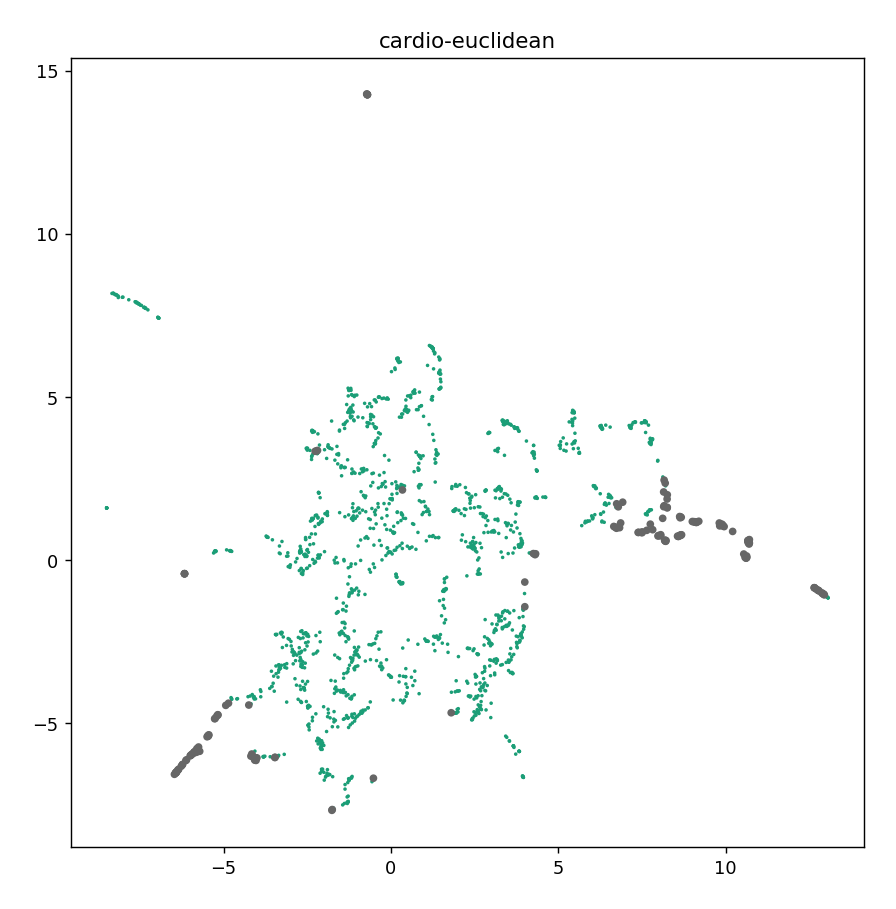
\includegraphics[width=2.5in]{images/umaps/cardio-euclidean-umap2d.png}
   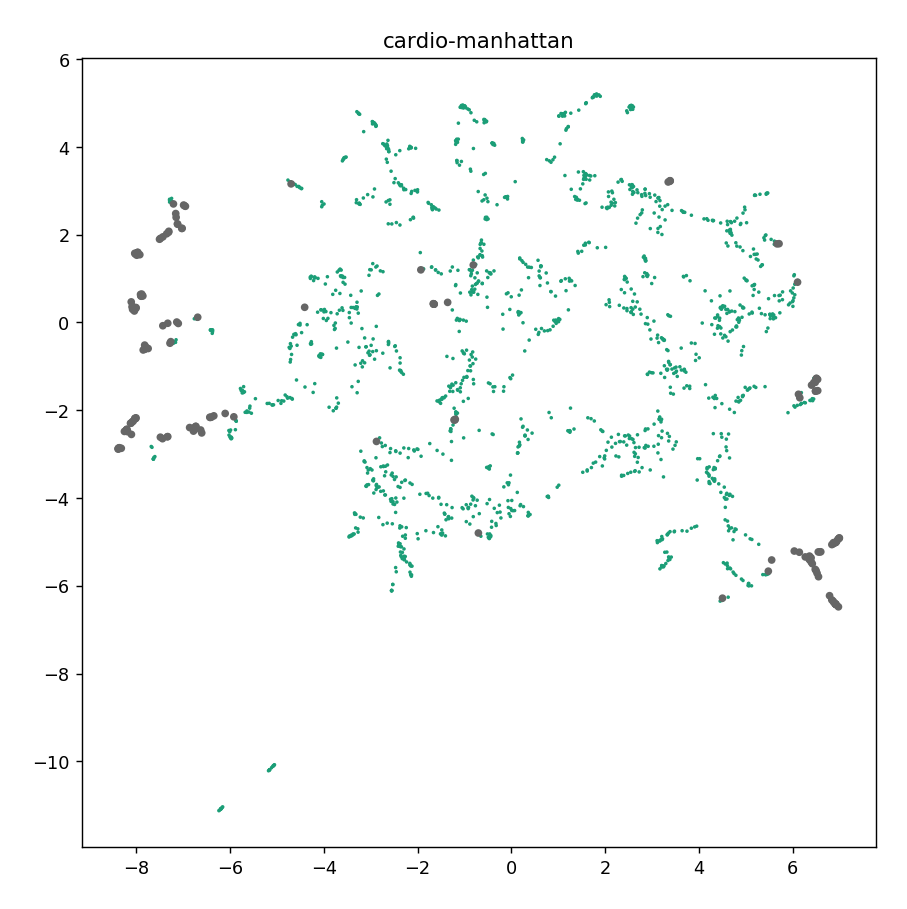
\includegraphics[width=2.5in]{images/umaps/cardio-manhattan-umap2d.png}
   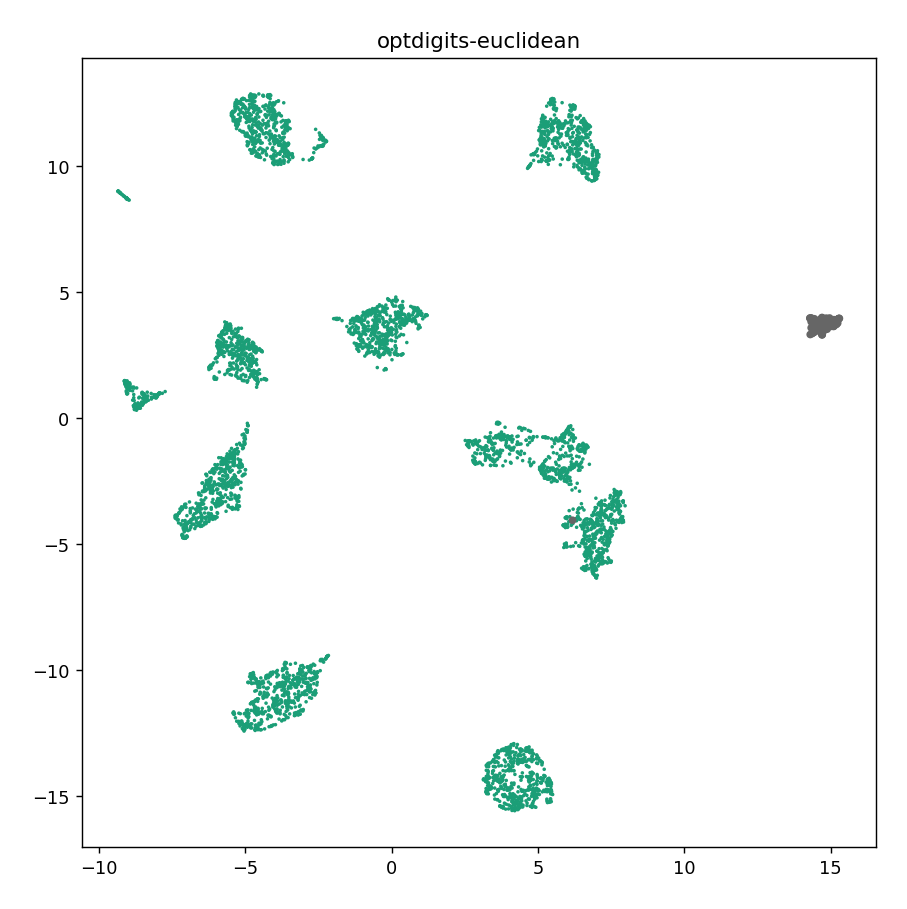
\includegraphics[width=2.5in]{images/umaps/optdigits-euclidean-umap2d.png}
   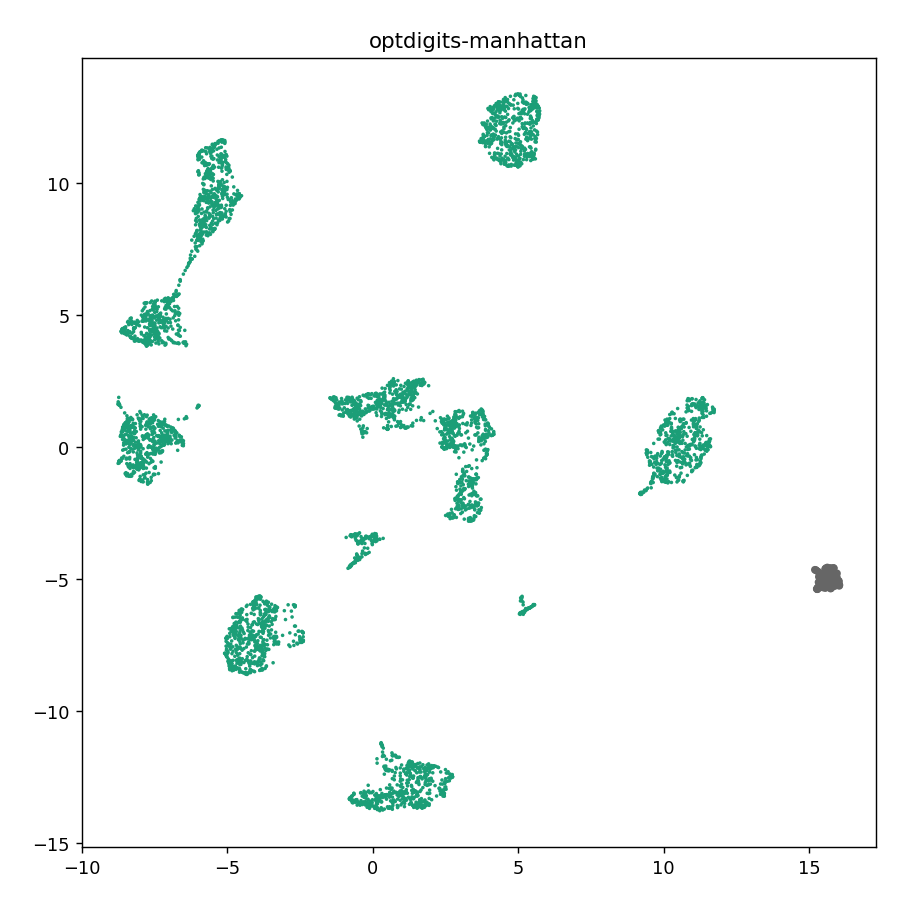
\includegraphics[width=2.5in]{images/umaps/optdigits-manhattan-umap2d.png}
   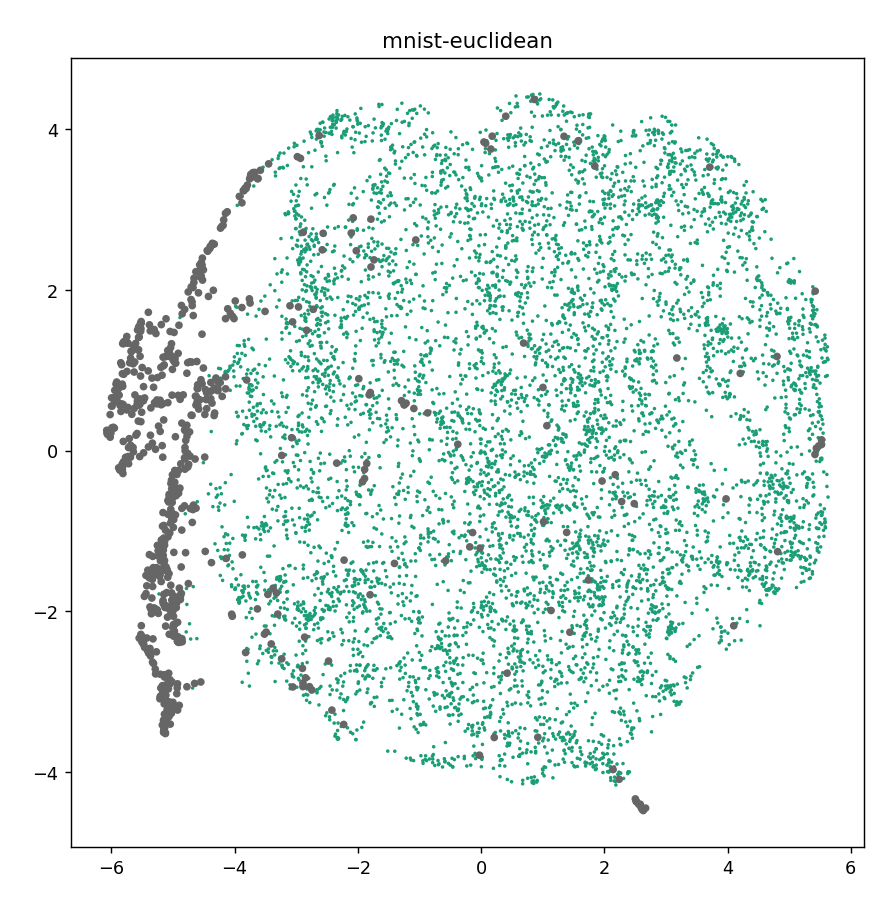
\includegraphics[width=2.5in]{images/umaps/mnist-euclidean-umap2d.png}
   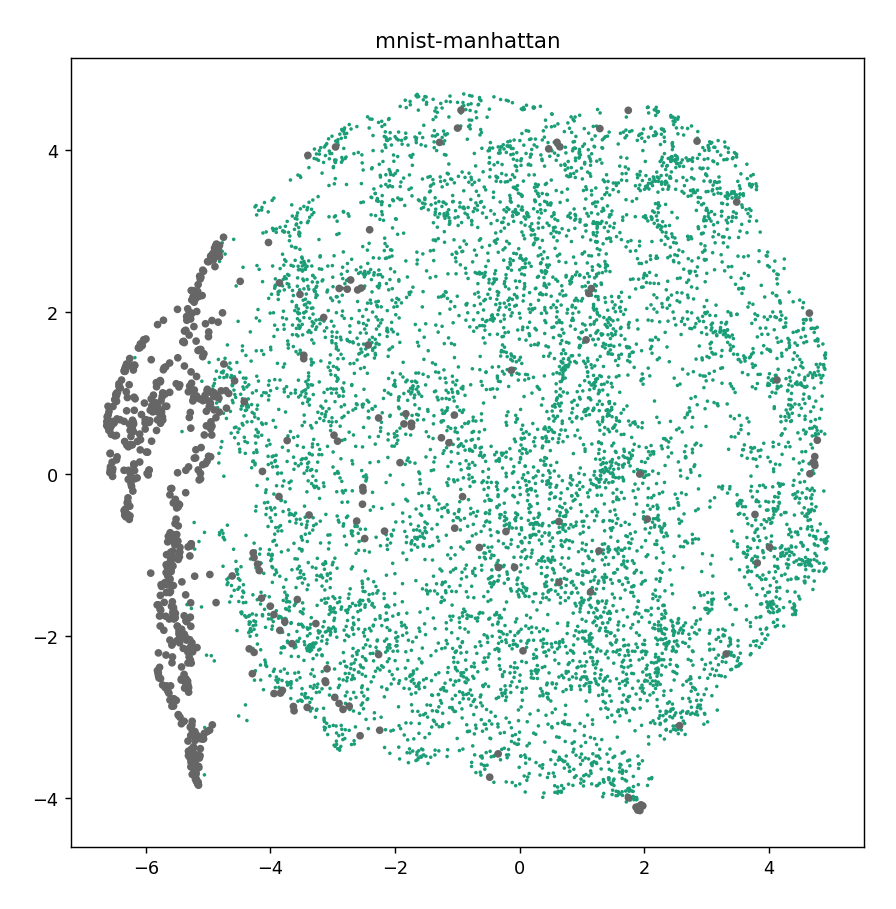
\includegraphics[width=2.5in]{images/umaps/mnist-manhattan-umap2d.png}
   \caption{UMAP projections of Cardio (first row), Optdigits (second row) and Mnist (third row).
   The distance metrics used are Euclidean (left column) and Manhattan (right column).
   Anomalies are in gray.
   Note that for MNIST, the UMAP projection does not find much structure, though most of the anomalies congregate to one side.
   For Cardio, there is a single main component to the manifold, and anomalies tend to be at the edges of that manifold.
   For OptDigits, there are several distinct pieces to the manifold, perhaps corresponding to different digits.
   Most algorithms perform comparably on MNIST, while CHAODA outperforms others on Cardio and OptDigits.}
   \label{supplement:fig:conclusions:umap-embeddings-1}
\end{figure*}

In Figure~\ref{supplement:fig:conclusions:umap-embeddings-2}, we show UMAP visualizations of the Pima dataset.
The inliers and outliers seem inseparable, and so all the methods perform poorly.

\begin{figure*}
   \centering
   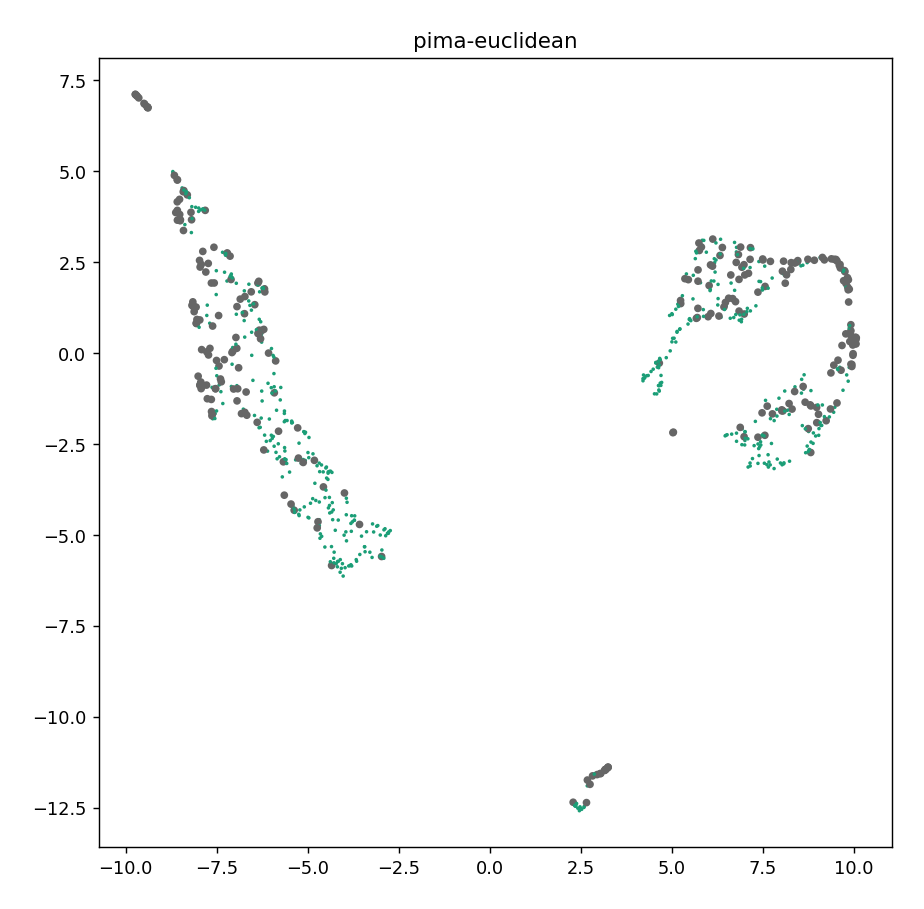
\includegraphics[width=2.5in]{images/umaps/pima-euclidean-umap2d.png}
   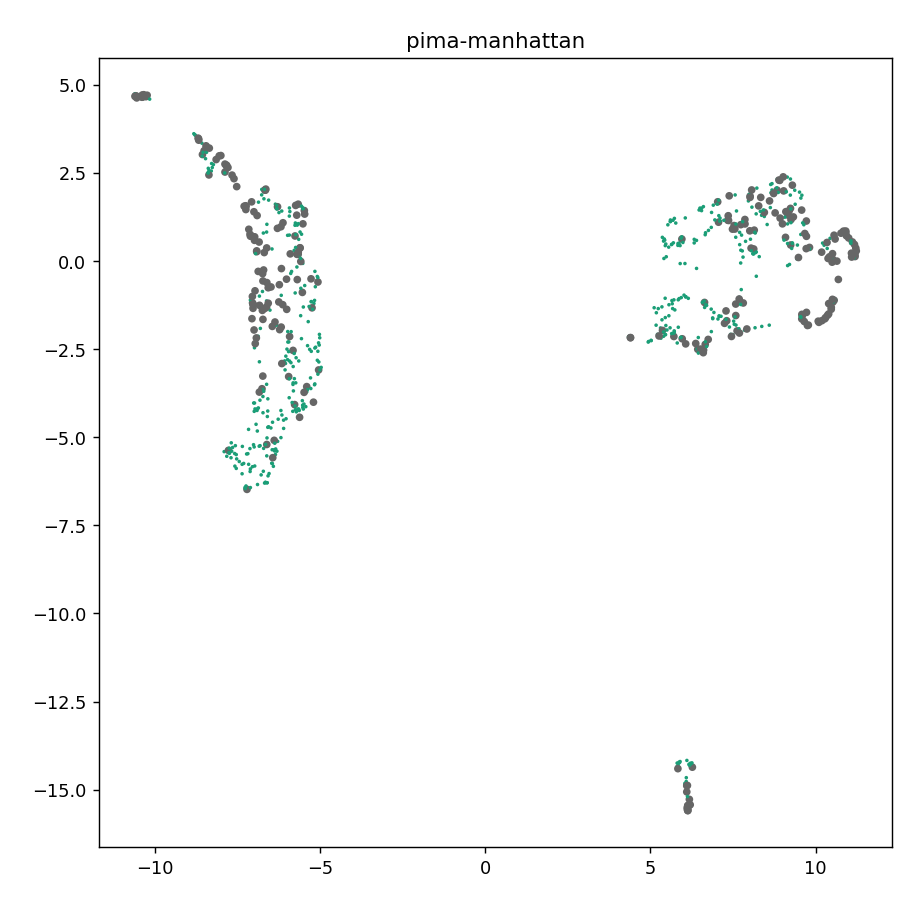
\includegraphics[width=2.5in]{images/umaps/pima-manhattan-umap2d.png}
   \caption{UMAP projections of the Pima dataset.
   All algorithms performed poorly on Pima.
   This may be because the anomalies and the outliers seem inseparable in the projection.}
   \label{supplement:fig:conclusions:umap-embeddings-2}
\end{figure*}


\section{Performance}
\label{supplement:sec:performance}

\subsection{Run-time performance on Test set of Datasets}

Tables~\ref{supplement:table:results:test-time-1}~and~\ref{supplement:table:results:test-time-2} report the running time, in seconds, of CHAODA and each competitor.
The fastest methods on each dataset are presented in bold face.


\begin{table*}[!t]
\renewcommand{\arraystretch}{1.15}
\caption{Time taken, in seconds, on the first half of the Test Datasets}
\label{supplement:table:results:test-time-1}
\vskip 0.15in
\begin{center}
\begin{small}
% \begin{sc}
\begin{tabular}{|c|c|c|c|c|c|c|c|c|c|}
\hline
\textbf{Model} & \textbf{Arrhy} & \textbf{BreastW} & \textbf{Cardio} & \textbf{Cover} & \textbf{Glass} & \textbf{Http} & \textbf{Iono} & \textbf{Lympho} & \textbf{Mammo} \\
\hline
CHAODA-fast &                6.70 &             4.71 &          135.17 &        1e3 &           1.06 &        119.14 &                2.64 &            1.08 &          46.42 \\
\hline
CHAODA &                6.90 &             4.80 &          143.31 &        3e3 &           1.10 &        221.81 &                2.78 &            1.74 &          71.54 \\
\hline
ABOD &                0.34 &             0.20 &            0.72 &          24.02 &  \textbf{0.07} &         19.08 &                0.13 &   \textbf{0.05} &           3.82 \\
\hline
AutoEncoder &                8.00 &             6.18 &            9.05 &         183.70 &           3.99 &        154.20 &                4.99 &            3.79 &          35.26 \\
\hline
CBLOF &                0.16 &             0.13 &            0.17 &    \textit{EX} &  \textbf{0.06} &   \textit{EX} &       \textbf{0.07} &   \textbf{0.05} &           0.20 \\
\hline
COF &                1.24 &             1.84 &           12.63 &       2e4 &           0.24 &      2e5 &                0.60 &            0.14 &         513.46 \\
\hline
HBOS &       \textbf{0.08} &    \textbf{0.00} &   \textbf{0.01} &           1.13 &  \textbf{0.00} & \textbf{0.01} &       \textbf{0.01} &   \textbf{0.01} &  \textbf{0.01} \\
\hline
IFOREST &                0.43 &             0.34 &            0.43 &           4.61 &           0.30 &          3.95 &                0.33 &            0.30 &           0.95 \\
\hline
KNN &                0.19 &    \textbf{0.07} &            0.30 &          11.46 &  \textbf{0.02} &          7.47 &       \textbf{0.05} &   \textbf{0.02} &           1.58 \\
\hline
LMDD &               14.85 &             2.62 &           22.12 &       1e4 &           0.57 &       4e3 &                1.73 &            0.42 &         243.01 \\
\hline
LOCI &              307.04 &      \textit{TO} &     \textit{TO} &    \textit{TO} &          25.68 &   \textit{TO} &              120.92 &            9.78 &    \textit{TO} \\
\hline
LODA &       \textbf{0.04} &    \textbf{0.03} &   \textbf{0.05} &           0.81 &  \textbf{0.03} &          0.66 &       \textbf{0.03} &   \textbf{0.03} &           0.17 \\
\hline
LOF &                0.16 &    \textbf{0.01} &            0.18 &          10.24 &  \textbf{0.00} &          1.93 &       \textbf{0.01} &   \textbf{0.00} &           0.59 \\
\hline
MCD &                5.08 &             0.64 &            0.89 &          28.65 &  \textbf{0.05} &          8.21 &                0.15 &   \textbf{0.05} &           2.11 \\
\hline
MOGAAL &               46.46 &            42.09 &          116.73 &    \textit{TO} &          40.67 &   \textit{TO} &               40.86 &           37.84 &    \textit{TO} \\
\hline
OCSVM &       \textbf{0.10} &    \textbf{0.02} &            0.23 &         257.95 &  \textbf{0.00} &        257.28 &       \textbf{0.01} &   \textbf{0.00} &           6.37 \\
\hline
SOD &                1.19 &             1.89 &           13.39 &    \textit{TO} &           0.31 &   \textit{TO} &                0.76 &            0.20 &         521.25 \\
\hline
SOGAAL &                6.70 &             5.03 &           14.43 &         591.14 &           3.95 &        597.17 &                4.71 &            3.96 &          92.27 \\
\hline
SOS &                0.69 &            47.40 &            4.11 &    \textit{TO} &           0.18 &   \textit{TO} &                0.33 &            0.11 &    \textit{TO} \\
\hline
VAE &               10.00 &             7.75 &           10.89 &         223.09 &           5.27 &        175.59 &                6.66 &            5.21 &          40.87 \\
\hline
\end{tabular}
% \end{sc}
\end{small}
\end{center}
\vskip -0.1in
\end{table*}


\begin{table*}[!t]
\renewcommand{\arraystretch}{1.15}
\caption{Time taken, in seconds, on the second half of the Test Datasets}
\label{supplement:table:results:test-time-2}
\vskip 0.15in
\begin{center}
\begin{small}
% \begin{sc}
\begin{tabular}{|c|c|c|c|c|c|c|c|c|c|}
\hline
\textbf{Model} & \textbf{Must} & \textbf{OptDigits} & \textbf{Pima} & \textbf{SatImg-2} & \textbf{Smtp} & \textbf{Vert} & \textbf{Vowels} &  \textbf{WBC} & \textbf{Wine} \\
\hline
CHAODA-fast &        858.15 &            3e3 &         12.36 &              358.49 &        272.61 &               1.88 &          123.34 &          5.26 &          0.39 \\
\hline
CHAODA &        982.25 &            6e3 &         13.50 &              611.14 &        451.74 &               2.21 &          181.91 &          6.10 &          0.40 \\
\hline
ABOD &          4.39 &               6.81 &          0.26 &                3.20 &         18.00 &      \textbf{0.08} &            0.51 &          0.14 & \textbf{0.04} \\
\hline
AutoEncoder &         23.40 &              24.29 &          4.65 &               23.73 &        195.61 &               2.85 &            6.98 &          4.70 &          3.31 \\
\hline
CBLOF &          0.27 &               0.44 & \textbf{0.08} &                0.31 &          0.65 &      \textbf{0.06} &   \textbf{0.10} & \textbf{0.08} & \textbf{0.05} \\
\hline
COF &         45.60 &             119.57 &          2.40 &              141.84 &      2e4 &               0.28 &            8.06 &          0.68 &          0.11 \\
\hline
HBOS & \textbf{0.07} &      \textbf{0.04} & \textbf{0.00} &       \textbf{0.02} & \textbf{0.01} &      \textbf{0.00} &   \textbf{0.01} & \textbf{0.01} & \textbf{0.00} \\
\hline
IFOREST &          0.93 &               0.92 &          0.35 &                0.79 &          3.90 &               0.30 &            0.40 &          0.33 &          0.29 \\
\hline
KNN &          3.50 &               5.53 & \textbf{0.09} &                1.84 &          6.83 &      \textbf{0.03} &            0.18 & \textbf{0.05} & \textbf{0.01} \\
\hline
LMDD &        375.11 &             421.22 &          2.86 &              302.94 &       4e3 &               0.59 &            9.47 &          1.91 &          0.33 \\
\hline
LOCI &   \textit{TO} &        \textit{TO} &   \textit{TO} &         \textit{TO} &   \textit{TO} &              35.97 &     \textit{TO} &        154.49 &          6.84 \\
\hline
LODA & \textbf{0.07} &      \textbf{0.10} & \textbf{0.04} &       \textbf{0.10} &          0.73 &      \textbf{0.03} &   \textbf{0.05} & \textbf{0.04} & \textbf{0.03} \\
\hline
LOF &          3.59 &               5.49 & \textbf{0.02} &                1.50 &          1.36 &      \textbf{0.00} &   \textbf{0.06} & \textbf{0.01} & \textbf{0.00} \\
\hline
MCD &         84.74 &               7.24 &          0.69 &                6.83 &         13.78 &      \textbf{0.05} &            0.81 &          0.11 & \textbf{0.05} \\
\hline
MOGAAL &        267.93 &             415.02 &         40.89 &              463.18 &   \textit{TO} &              39.86 &           80.35 &         40.65 &         38.10 \\
\hline
OCSVM &          2.51 &               3.71 & \textbf{0.03} &                3.14 &        252.52 &      \textbf{0.00} &            0.11 & \textbf{0.01} & \textbf{0.00} \\
\hline
SOD &         56.94 &             131.49 &          2.48 &              210.39 &   \textit{TO} &               0.54 &           13.92 &          1.03 &          0.19 \\
\hline
SOGAAL &         29.55 &              44.72 &          5.20 &               48.79 &        592.27 &               4.69 &           10.38 &          4.76 &          4.01 \\
\hline
SOS &          9.37 &              26.09 &          1.01 &               34.96 &   \textit{TO} &               0.21 &            2.81 &          0.36 & \textbf{0.10} \\
\hline
VAE &         30.38 &              30.58 &          5.67 &               30.41 &        176.84 &               4.03 &           10.46 &          5.33 &          4.62 \\
\hline
\end{tabular}
% \end{sc}
\end{small}
\end{center}
\vskip -0.1in
\end{table*}


\subsection{AUC and Runtime performance on Train set of Datasets}

Tables~\ref{supplement:table:results:train-performance}~and~\ref{supplement:table:results:train-time} report the  the AUC performance and running time, respectively, of CHAODA and each competitor on the train set of datasets.

\begin{table*}[!t]
\renewcommand{\arraystretch}{1.25}
\caption{Performance on Train Datasets}
\label{supplement:table:results:train-performance}
% \centering
\vskip 0.15in
\begin{center}
\begin{small}
% \begin{sc}
\begin{tabular}{|c|c|c|c|c|c|c|}
\hline
\textbf{Model} & \textbf{Annthy} & \textbf{Mnist} & \textbf{PenDigits} & \textbf{Satellite} & \textbf{Shuttle} & \textbf{Thyroid} \\
\hline
CHAODA-fast &                0.64 &  \textbf{0.78} &      \textbf{0.94} &      \textbf{0.79} &             0.51 &    \textbf{0.89} \\
\hline
CHAODA &                0.65 &           0.73 &      \textbf{0.95} &               0.73 &             0.85 &    \textbf{0.89} \\
\hline
ABOD &                0.50 &           0.60 &               0.53 &               0.51 &             0.54 &             0.50 \\
\hline
AutoEncoder &                0.69 &           0.67 &               0.58 &               0.63 &             0.94 &             0.88 \\
\hline
CBLOF &                0.59 &           0.62 &               0.59 &               0.68 &    \textbf{0.99} &             0.87 \\
\hline
COF &                0.59 &           0.56 &               0.53 &               0.56 &             0.52 &             0.49 \\
\hline
HBOS &       \textbf{0.84} &           0.53 &               0.52 &               0.62 &             0.74 &             0.86 \\
\hline
IFOREST &                0.70 &           0.61 &               0.63 &               0.70 &             0.91 &    \textbf{0.91} \\
\hline
KNN &                0.65 &           0.65 &               0.51 &               0.56 &             0.53 &             0.56 \\
\hline
LMDD &                0.52 &           0.59 &               0.56 &               0.42 &             0.92 &             0.70 \\
\hline
LOCI &         \textit{TO} &    \textit{TO} &        \textit{TO} &        \textit{TO} &      \textit{TO} &      \textit{TO} \\
\hline
LODA &                0.63 &           0.66 &               0.57 &               0.65 &             0.96 &    \textbf{0.90} \\
\hline
LOF &                0.60 &           0.57 &               0.52 &               0.57 &             0.53 &             0.49 \\
\hline
MCD &                0.72 &           0.57 &               0.53 &               0.58 &             0.96 &             0.85 \\
\hline
MOGAAL &                0.46 &    \textit{TO} &               0.67 &               0.59 &      \textit{TO} &             0.49 \\
\hline
OCSVM &                0.62 &           0.63 &               0.59 &               0.62 &    \textbf{0.97} &             0.78 \\
\hline
SOD &                0.64 &           0.55 &               0.52 &               0.52 &      \textit{TO} &             0.53 \\
\hline
SOGAAL &                0.46 &           0.57 &               0.57 &               0.60 &             0.96 &             0.49 \\
\hline
SOS &                0.50 &           0.52 &               0.52 &               0.47 &      \textit{TO} &             0.50 \\
\hline
VAE &                0.69 &           0.67 &               0.58 &               0.63 &             0.94 &             0.88 \\
\hline
\end{tabular}
% \end{sc}
\end{small}
\end{center}
\vskip -0.1in
\end{table*}

\begin{table*}[!t]
\renewcommand{\arraystretch}{1.25}
\caption{Time taken, in seconds, on Train Datasets}
\label{supplement:table:results:train-time}
\centering
\begin{tabular}{|c|c|c|c|c|c|c|}
\hline
\textbf{Model} & \textbf{Annthy} & \textbf{Mnist} & \textbf{PenDigits} & \textbf{Satellite} & \textbf{Shuttle} & \textbf{Thyroid} \\
\hline
CHAODA-fast &              161.85 &        6e3 &             617.93 &             425.03 &             5.48 &           117.97 \\
\hline
CHAODA &              205.74 &       1e4 &             771.89 &             891.19 &         2e4 &           219.32 \\
\hline
ABOD &                3.42 &          16.39 &               2.83 &               3.53 &            21.58 &             1.25 \\
\hline
AutoEncoder &               22.80 &          40.54 &              23.87 &              26.74 &           158.72 &            12.84 \\
\hline
CBLOF &                1.01 &           1.14 &               0.23 &               0.30 &             0.71 &             0.21 \\
\hline
COF &              215.63 &         277.91 &             199.03 &             176.35 &         1e4 &            54.82 \\
\hline
HBOS &                1.58 &  \textbf{0.06} &      \textbf{0.01} &      \textbf{0.02} &    \textbf{0.03} &    \textbf{0.00} \\
\hline
IFOREST &                0.73 &           1.41 &               0.80 &               0.84 &             3.24 &             0.54 \\
\hline
KNN &                0.84 &          14.30 &               1.25 &               2.05 &             9.13 &             0.42 \\
\hline
LMDD &              107.05 &        1e3 &             197.48 &             371.63 &          6e3 &            32.69 \\
\hline
LOCI &         \textit{TO} &    \textit{TO} &        \textit{TO} &        \textit{TO} &      \textit{TO} &      \textit{TO} \\
\hline
LODA &                0.13 &           0.13 &               0.12 &               0.11 &             0.59 &    \textbf{0.08} \\
\hline
LOF &                0.26 &          14.79 &               0.90 &               1.71 &             6.30 &    \textbf{0.09} \\
\hline
MCD &                1.50 &          20.56 &               3.01 &              10.39 &            10.78 &             1.03 \\
\hline
MOGAAL &              594.69 &    \textit{TO} &             561.40 &             513.84 &      \textit{TO} &           280.80 \\
\hline
OCSVM &                2.70 &          11.30 &               3.04 &               3.83 &           162.18 &             0.68 \\
\hline
SOD &              262.80 &         281.86 &             195.81 &             253.71 &      \textit{TO} &            91.48 \\
\hline
SOGAAL &               61.14 &          68.03 &              55.40 &              50.07 &           460.66 &            31.43 \\
\hline
SOS &              101.82 &          54.22 &              46.02 &              42.62 &      \textit{TO} &            42.10 \\
\hline
VAE &               27.95 &          50.16 &              29.63 &              33.51 &           182.23 &            16.18 \\
\hline
\end{tabular}
\end{table*}


\bibliographystyle{icml2021}
\bibliography{references}

\end{document}